\documentclass{article}

\usepackage{graphicx}
\usepackage{tikz}
\usepackage{tikzsymbols}
\usetikzlibrary{calc,patterns,shapes.geometric}
\pagestyle{empty}
\usepackage[margin=0pt]{geometry}
\geometry{papersize={14in,12in}}

\def\centerarc[#1](#2)(#3:#4:#5){\draw[#1] ($(#2)+({#5*cos(#3)},{#5*sin(#3)})$) arc (#3:#4:#5);}

\begin{document}
	\begin{figure}
		\centering
		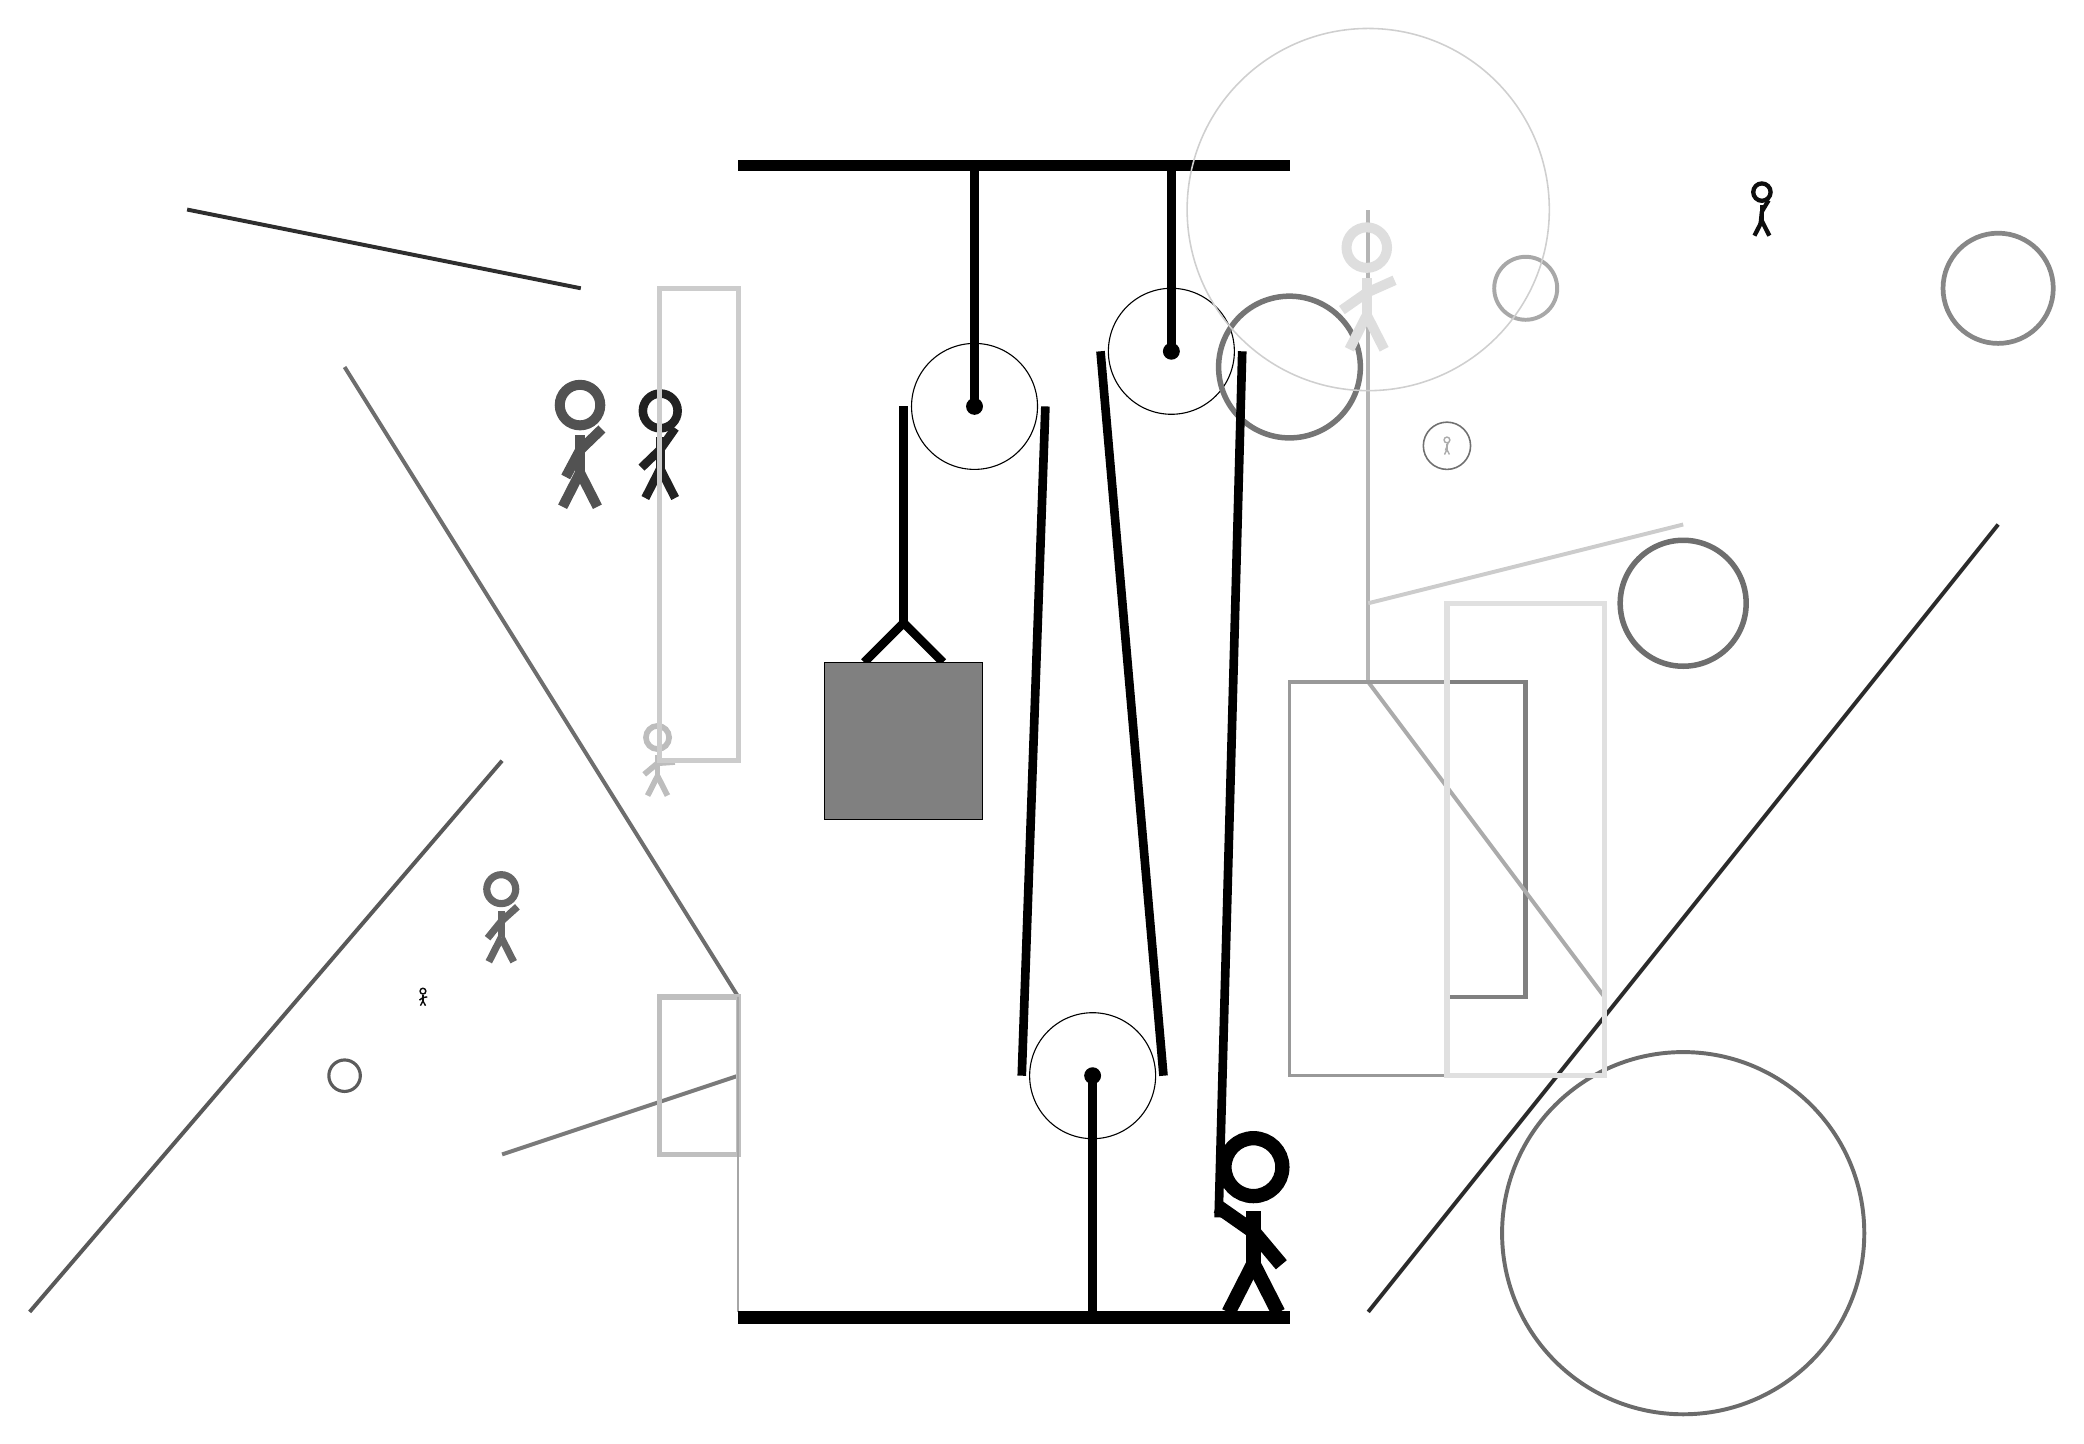
\begin{tikzpicture}
			%%%%% START %%%%%
			
			\draw[fill=black] (-2, 11.5) rectangle (5, 11.625);
			
			\draw (1, 8.5) circle (0.8);
			\draw[fill=black] (1, 8.5) circle (0.1);
			\draw[line width=1.1mm]  (1, 11.5) -- (1, 8.5);
			
			\draw[fill=white](2.5, 0.0) circle (0.8);
			\draw[fill=black] (2.5, 0.0) circle (0.1);
			\draw[line width=1.1mm]  (2.5, -3) -- (2.5, 0.0);
			
			\draw[fill=white](3.5, 9.2) circle (0.8);
			\draw[fill=black] (3.5, 9.2) circle (0.1);
			\draw[line width=1.1mm] (3.5, 11.5) -- (3.5, 9.2);
			
			\draw[line width=1.1mm] (-0.4, 5.25) -- (0.1, 5.75) -- (0.6, 5.25);
			\draw[fill=black!50] (-0.9, 5.25) rectangle (1.1, 3.25);
			
			\draw[line width=0.6mm, color=black!50] (7, 5) rectangle (8, 1);
			
			\node[line width=0.4mm, color=black!26] at (-3, 4) {\Strichmaxerl[4][40][4]};
			\draw[line width=0.5mm, color=black!83](6, -3) -- (14, 7);
			\draw [line width=0.5mm, color=black!58](10, -2) circle (2.3);
			\node[line width=0.7mm, color=black!95] at (11, 11) {\Strichmaxerl[3][84][59]};
			\draw[line width=0.5mm, color=black!52](-5, -1) -- (-2, 0);
			
			\draw[line width=0.5mm, color=black!33](9, 1) -- (6, 5);
			
			\draw[line width=0.5mm, color=black!29](6, 5) -- (6, 11);
			\node[line width=0.5mm, color=black!95] at (-6, 1) {\Strichmaxerl[1][36][9]};
			\node[line width=0.5mm, color=black!87] at (-3, 8) {\Strichmaxerl[6][44][55]};
			\draw [line width=0.7mm, color=black!54](5, 9) circle (0.9);
			
			\draw [line width=0.5mm, color=black!34](8, 10) circle (0.4);
			\node[line width=0.7mm, color=black!33] at (7, 8) {\Strichmaxerl[1][69][72]};
			
			\draw[line width=0.5mm, color=black!82](-4, 10) -- (-9, 11);
			\draw [line width=0.2mm, color=black!19](6, 11) circle (2.3);
			\draw[line width=0.5mm, color=black!20](10, 7) -- (6, 6);
			
			\draw[line width=0.6mm, color=black!20] (-3, 4) rectangle (-2, 10);
			
			\node[line width=0.4mm, color=black!68] at (-4, 8) {\Strichmaxerl[7][62][44]};
			\draw[line width=0.5mm, color=black!57](-7, 9) -- (-2, 1);
			\draw[line width=0.7mm, color=black!25] (-2, 1) rectangle (-3, -1);
			\draw[line width=0.4mm, color=black!40] (7, 5) rectangle (5, 0);
			
			\draw[line width=0.7mm, color=black!12] (7, 6) rectangle (9, 0);
			\draw [line width=0.6mm, color=black!47](14, 10) circle (0.7);
			\node[line width=0.7mm, color=black!60] at (-5, 2) {\Strichmaxerl[5][51][42]};
			\draw [line width=0.7mm, color=black!57](10, 6) circle (0.8);
			\node[line width=0.7mm, color=black!13] at (6, 10) {\Strichmaxerl[7][35][24]};
			\draw [line width=0.2mm, color=black!56](7, 8) circle (0.3);
			\draw [line width=0.4mm, color=black!64](-7, 0) circle (0.2);
			
			\draw[line width=0.5mm, color=black!65](-5, 4) -- (-11, -3);
			
			\draw[line width=0.3mm, color=black!35] (-2, 1) rectangle (-2, -3);
			
			\draw[line width=1.1mm] (0.1, 8.5) -- (0.1, 5.75);
			\centerarc[line width=1.1mm](1, 8.5)(0:180:0.9);
			\draw[line width=1.1mm](1.9, 8.5) -- (1.6, 0.0);
			\centerarc[line width=1.1mm](2.5, 0.0)(180:360:0.9);
			\draw[line width=1.1mm](3.4, 0.0) -- (2.6, 9.2);
			\centerarc[line width=1.1mm](3.5, 9.2)(0:180:0.9);
			\draw[line width=1.1mm](4.4, 9.2) -- (4.1, -1.8);
			
			\node at (4.5, -1.9) {\Strichmaxerl[10][-35][-50]};
			
			\draw[fill=black] (-2, -3) rectangle (5, -3.15);
			
			%%%%% END %%%%%
		\end{tikzpicture}
	\end{figure}	
\end{document}